\documentclass[12pt, a4paper]{article}
\usepackage[utf8]{inputenc}
%\usepackage[french]{babel}
\usepackage{amsfonts}
\usepackage{graphicx}
\usepackage{fancyhdr}
\usepackage{url}
\usepackage[usenames,dvipsnames]{color}

\usepackage[top=3.3cm, bottom=3.3cm, left=2cm, right=2cm]{geometry}

\renewcommand{\baselinestretch}{1.2}

\pagestyle{fancy}
\usepackage{lastpage}
\renewcommand\headrulewidth{1pt}
\fancyhead[L]{Image UpScaling}
\fancyhead[R]{INSA de Rouen}
\renewcommand\footrulewidth{1pt}
\fancyfoot[C]{\textbf{Page \thepage/\pageref{LastPage}}}
\fancyfoot[R]{
\includegraphics[width=0.10\textwidth]{Images/Logo_INSA.png}}

\title{Rapport de projet}
\author{Ophélie Guenoux \\Olivier Petit}
\date{Janvier 2016}

\begin{document}

\makeatletter
\begin{titlepage}
  \begin{center}
      
\includegraphics[width=0.20\textwidth]{Images/Logo_INSA.png}
      \hfill
      
\includegraphics[width=0.25\textwidth]{Images/logoasi.png}\\
    \vspace{1cm}
		\Huge \underline{\@title} 
			\\ \textsc{Image UpScaling}
			\\ \Large Projet d'Approfondissement et d'Ouverture
			\vspace{1cm}
			\begin{figure}[h!]
				\centering
				%\includegraphics[width=0.7\textwidth]{Images/radcul.jpg}
			\end{figure}
	\vspace{1cm}
	\end{center}
	\raggedright
	\large Ophélie Guenoux \hfill Encadrant : M.Chatelain \& M.Herault
	\\Olivier Petit \hfill INSA Rouen ASI4
	
\end{titlepage}

\newpage
\tableofcontents
\newpage
\section*{Introduction}

\section{État de l'art}

\subsection{Image Scaling}
L'\textit{image scaling} est l'expression anglaise désignant les procédés informatiques liés à l'agrandissement ou la réduction de la taille d'une image.

Il existe deux familles d'image, les images vectoriels et les images matriciels. Dans le cas d'images vectoriels l'agrandissement et la réduction sont effectués par le recalcul de l'images à partir d'équations stockées dans le fichier. De cette manière nous pouvons obtenir une image lisse quelque soit le coefficient d'échelle appliqué. Ce recalcul est cependant coûteux en temps et ressources. C'est la raison pour laquelle les images matriciel sont plus répandues. Ce type d'image consiste simplement en une matrice de trois dimensions, pour la largeur, la hauteur, et les trois ou quatre canaux de couleurs. Des algorithmes de compressions permettent de faciliter le stockage mais aussi la transmission car dans le cas contraire les images peuvent être assez "lourdes".

Dans de nombreuses application les images matriciels sont préférées. Par exemple dans les anciens jeux-vidéos, les icônes, et toutes les images généralement sur internet. Là où les temps de chagement doivent être minimum.

Cependant il peut être intéressant de vouloir modifier la taille d'une image pour s'adapter par exemple aux différents types d'écrans. De plus avec l'augmentation de la résolution des écrans, certaines images doivent être très petites pour être affichées correctement. Le meilleur exemple étant la remasterisation d'anciens jeux vidéos.

\begin{figure}[h!]
  \centering
  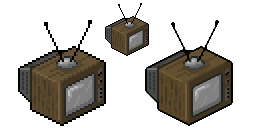
\includegraphics[scale=0.7]{Images/tele.png}
  \caption{Upscaling x2}
\end{figure}

\subsection{Agrandissement}
 
L'augmentation de la taille d'une image revient à "créer" de nouveaux pixels qu'il faudrait remplir le mieux possible afin de garder une continuité.

L'algorithme le plus simple est celui du plus proche voisin. Il est très rapide mais fourni un résultat pixélisé 

\begin{figure}[h!]
  \centering
  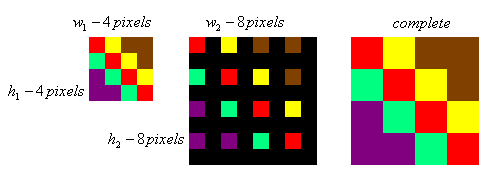
\includegraphics[scale=0.6]{Images/plus_proche_voisin.png}
  \caption{Algorithme du plus proche voisin}
\end{figure}

De très nombreux algorithme existent, certain développés par de très grands laboratoires. Une liste exhaustive est diposible ici

\url{https://en.wikipedia.org/wiki/Image_scaling#Pixel_art_scaling_algorithms}

\subsection{Réduction}

La réduction d'une image est un procédé plus simple car il consiste généralement à supprimer des pixels régulièrement (par exemple un sur deux).


\section{Choix de la librairie}
Pour notre projet, nous souhaitions agrandir des images avec un réseau de neurones. De ce fait, nous avons commencé à nous renseigner sur les différentes librairies. \\ Parmi elles, Pylearn2 qui nous avait été justement conseiller par nos encadrants. 
\subsection{Theano et Pylearn2}
Notre choix s'est donc orienté vers Pylearn2 une librairie opensource sous license BSD qui utilise Theano (librairie machine-learning reconnue).
\\ De plus, c'est une librairie python, langage que nous connaissions.
\\

Pylearn2 est avant tout une librairie de machine learning permettant de résoudre des problèmes de toutes sortes.(Clustering, classification, etc...)
\\De plus, la librairie implémente un ensemble de fonctions liées à la création de réseaux de neurones artificiels. Il s'agit de la classe MLP (\emph{multi layers perceptron}), qui contient toutes les types de couches connues. \\ Par exemple, dans le code suivant, nous créons un réseau de neurones contenant une couche de 75 neurones avec comme fonction d'activation une \emph{Sigmoid}
\begin{verbatim}
"model": !obj:pylearn2.models.mlp.MLP {
  "layers": [
   !obj:pylearn2.models.mlp.Sigmoid {
     layer_name: 'h1',
     dim: 75,
     irange: .5,
   },
 ]
}
\end{verbatim}
\subsection{Utilisation de \emph{YAML} avec Python}
Pylearn2 permet la définition d'un modèle de machine learning grâce à un script en \emph{YAML}.\\ L'exemple précédent est un extrait du script \emph{YAML} utilisé dans notre projet. 
\\

Initialement, pour bien comprendre le fonctionnement de la bibliothèque, nous avions réalisé une première version du projet uniquement avec des scripts Python. 
\\ Cependant, nous nous sommes très vite rendu compte des limites que cela engendrait. En effet, le code était devenu lourd et difficile à utiliser. 
\\

Par la suite, nous avons donc utilisé \emph{YAML} avec Python comme proposé par Pylearn2. Le côté architecture du réseau de neurones centralisé dans les scripts \emph{YAML} et le reste gérer par les scripts Python. 

\section{Les différentes étapes du projet}
	\subsection{Choix et construction du Dataset}
Au commencement du projet, il était question de faire un Dataset composé de chiffre allant de 0 à 9. 
Cependant, nous avons vite été confronté à un problème, sa taille. En effet, notre Dataset n'était composé que de 50 éléments, ce qui est largement insuffisant pour que l'apprentissage soit efficace.
\\ Nous avons donc décidé de changer les données utilisées en images 32 pixels par 32, noir et blanc, représentant des ellipses et des rectangles.
 
	\subsection{Utilisation de Patchs}
	% mettre des images en entier sur le réseau -> beaucoup trop lent. Du coup réduction de la taille du réseau en ne passant que les patchs
	% deux nouveaux algo pour découper l'image en patch et pour la reformer
	\subsection{Structure du réseau}
	% nb couche
	\subsubsection{Changement des fonctions d'activation}
	% erreur de domaine de nos données, SIgmoid prend entre -inf et +inf pour ressortir en 0 et 1 ; 
	% ajouter un shéma pour expliquer les différentes couches 
\section{Problèmes rencontrés}
	\subsection{Le problème du pas}
	% Avant nous baissions tout simplement le learning rate ds une certaines fourchette d'epochs
	% tente d'utiliser un algo plus "intelligent" qui regarde 1 channel +val de sortie et par rapport à cette valeur fait augmenter ou dim le LR
	\subsection{Upscalling-RGB}
	% tentative de faire un réseau de neurones capable de faire de l'upscalling avec des images en couleur. 
	% -> problème notre image de sortie est en niveau de bleu principalement

\section*{Conclusion}
\end{document}
